\documentclass[tikz,border=10pt]{standalone}
\usepackage{tikz}
\usetikzlibrary{shapes.geometric}
\usetikzlibrary{calc}

\begin{document}
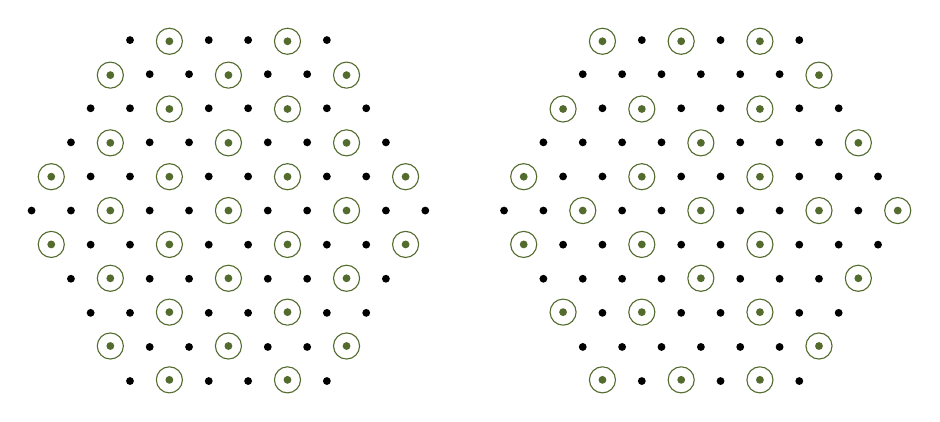
\begin{tikzpicture}[dot/.style={circle, fill=black, inner sep=1pt}]

%─────────────
% Controls
%─────────────
\def\hexstep{0.5}  % Distance from center to first ring point (controls scale)
\definecolor{olivegreen}{rgb}{0.33,0.42,0.18}  % Custom olive green

%─────────────────────────────────────────────────────────────
% Draws a hexagonal lattice of dots:
%─────────────────────────────────────────────────────────────
\newcommand{\drawHexagonDots}[3]{%
  \begin{scope}[shift={({#2},{#3})}]

    \pgfmathtruncatemacro{\rings}{#1}

    \ifnum\rings<1
      \node[dot] at (0,0) {};
    \else
      % Always draw the central dot at the origin
      \node[dot] at (0,0) {};

      % Loop over each ring from 1 to total number
      \foreach \r in {1,...,\rings} {
        \pgfmathsetmacro{\rad}{\r * \hexstep}  % Radius for this ring

        % Each ring has 6 sides (hexagon)
        \foreach \side in {0,...,5} {
          \pgfmathsetmacro{\angleA}{60*\side}
          \pgfmathsetmacro{\angleB}{60*(\side+1)}

          % Define endpoints of one hex side arc at current radius
          \coordinate (A) at (\angleA:\rad);
          \coordinate (B) at (\angleB:\rad);

          % Interpolate points between A and B
          \foreach \k in {0,...,\numexpr\r-1} {
            \pgfmathsetmacro{\t}{\k/\r}
            \path ($(A)!{\t}!(B)$) node[dot] {};
          }
        }
      }
    \fi
  \end{scope}
}

%─────────────
% Manually draw in selected nodes
%─────────────
\newcommand{\selectPoint}[2]{%
  \node[circle, draw=olivegreen, fill=white] at ({#1},{#2}) {}; 
  \node[dot, fill=olivegreen] at ({#1},{#2}) {}; 
}

% \newcommand{\selectPoint}[2]{%
%   \node[draw=olivegreen, fill=white, regular polygon, regular polygon sides=6, minimum size=28pt] at ({#1},{#2}) {}; 
%   \node[dot, fill=olivegreen] at ({#1},{#2}) {}; 
% }


% H_4 through H_5
%─────────────
% Draw examples H₁ through H₃
%─────────────
\drawHexagonDots{5}{-3}{0}     % H4 = 1
\drawHexagonDots{5}{3}{0}     % H5 = 7


%H_5
\selectPoint{-3}{0}
\selectPoint{-3}{-.86}
\selectPoint{-3}{.86}
\selectPoint{-3}{-1.72}
\selectPoint{-3}{1.72}
\selectPoint{-3.75}{-.43}
\selectPoint{-3.75}{.43}
\selectPoint{-3.75}{-1.29}
\selectPoint{-3.75}{1.29}
\selectPoint{-3.75}{-2.15}
\selectPoint{-3.75}{2.15}
\selectPoint{-2.25}{-.43}
\selectPoint{-2.25}{.43}
\selectPoint{-5.25}{-.43}
\selectPoint{-5.25}{.43}
\selectPoint{-.75}{-.43}
\selectPoint{-.75}{.43}
\selectPoint{-2.25}{-1.29}
\selectPoint{-2.25}{1.29}
\selectPoint{-2.25}{-2.15}
\selectPoint{-2.25}{2.15}
\selectPoint{-1.5}{0}
\selectPoint{-1.5}{-.86}
\selectPoint{-1.5}{.86}
\selectPoint{-1.5}{-1.72}
\selectPoint{-1.5}{1.72}
\selectPoint{-4.5}{0}
\selectPoint{-4.5}{-.86}
\selectPoint{-4.5}{.86}
\selectPoint{-4.5}{-1.72}
\selectPoint{-4.5}{1.72}

%H_5_2

\selectPoint{5.5}{0}
\selectPoint{1.75}{-2.15}
\selectPoint{2.75}{-2.15}
\selectPoint{3.75}{-2.15}
\selectPoint{1.75}{2.15}
\selectPoint{2.75}{2.15}
\selectPoint{3.75}{2.15}
\selectPoint{1.25}{-1.29}
\selectPoint{1.25}{1.29}
\selectPoint{.75}{-.43}
\selectPoint{.75}{.43}
\selectPoint{5}{-.86}
\selectPoint{5}{.86}
\selectPoint{4.5}{-1.72}
\selectPoint{4.5}{1.72}
\selectPoint{2.25}{-1.29}
\selectPoint{2.25}{1.29}
\selectPoint{2.25}{-.43}
\selectPoint{2.25}{.43}
\selectPoint{3.75}{-1.29}
\selectPoint{3.75}{1.29}
\selectPoint{3.75}{-.43}
\selectPoint{3.75}{.43}
\selectPoint{1.5}{0}
\selectPoint{4.5}{0}
\selectPoint{3}{0}
\selectPoint{3}{.86}
\selectPoint{3}{-.86}
% \selectPoint{1.75}{1.29}
% \selectPoint{2.75}{1.29}
% \selectPoint{3.75}{1.29}
% \selectPoint{1.75}{-.43}
% \selectPoint{2.75}{-.43}
% \selectPoint{3.75}{-.43}
% \selectPoint{1.75}{.43}
% \selectPoint{2.75}{.43}
% \selectPoint{3.75}{.43}

% \selectPoint{1}{0}
% \selectPoint{2}{0}
% \selectPoint{4}{0}
% \selectPoint{5}{0}
% \selectPoint{4}{-1.72}
% \selectPoint{4}{1.72}
% \selectPoint{2}{-1.72}
% \selectPoint{2}{1.72}
% \selectPoint{3}{-1.72}
% \selectPoint{3}{1.72}
% % \selectPoint{3}{-.86}
% \selectPoint{3.5}{-.86}
% \selectPoint{2.5}{-.86}
% \selectPoint{3.5}{.86}
% \selectPoint{2.5}{.86}
% \selectPoint{1.5}{-.86}
% \selectPoint{1.5}{.86}
% \selectPoint{4.5}{-.86}
% \selectPoint{4.5}{.86}

% \selectPoint{3.75}{-.43}
% \selectPoint{3.75}{.43}
% \selectPoint{3.75}{-1.29}
% \selectPoint{3.75}{1.29}
% \selectPoint{2.25}{-.43}
% \selectPoint{2.25}{.43}
% \selectPoint{2.25}{-1.29}
% \selectPoint{2.25}{1.29}
% \selectPoint{1.5}{0}
% \selectPoint{1.5}{-.86}
% \selectPoint{1.5}{.86}
% \selectPoint{4.5}{0}
% \selectPoint{4.5}{-.86}
% \selectPoint{4.5}{.86}
% \selectPoint{-4.5}{0}
% %H_1
% \selectPoint{-1.5}{0}
% \selectPoint{-2.25}{-.43}
% \selectPoint{-2.25}{.43}
% %H_2
% \selectPoint{1}{0}
% \selectPoint{2}{0}
% \selectPoint{0}{0}
% \selectPoint{1.5}{-0.86}
% \selectPoint{1.5}{0.86}
% \selectPoint{0.5}{-0.86}
% \selectPoint{0.5}{0.86}
% %H_3
% \selectPoint{4.75}{0}
% \selectPoint{5.5}{-.43}
% \selectPoint{5.5}{.43}
% \selectPoint{3.25}{0}
% \selectPoint{6.25}{0}
% \selectPoint{4}{1.29}
% \selectPoint{4}{-1.29}
% \selectPoint{5.5}{1.29}
% \selectPoint{5.5}{-1.29}
% \selectPoint{4}{.43}
% \selectPoint{4}{-.43}
% \selectPoint{4.75}{.86}
% \selectPoint{4.75}{-.86}
% % Bad method below 
% % \selectPoint{5.25}{0}
% % \selectPoint{4.5}{-.43}
% % \selectPoint{4.5}{.43}
% % \selectPoint{6.25}{0}
% % \selectPoint{4}{1.29}
% % \selectPoint{4}{-1.29}
% % \selectPoint{5}{1.29}
% % \selectPoint{5}{-1.29}
% % \selectPoint{3.5}{.43}
% % \selectPoint{3.5}{-.43}
% % \selectPoint{5.75}{.86}
% % \selectPoint{5.75}{-.86}

% %─────────────
% % Labels
% %─────────────
% \node at (-4.5,-2) {$H_0 \mapsto C_1$};
% \node at (-2,-2) {$H_1 \mapsto C_2$};
% \node at ( 1,-2) {$H_2 \mapsto C_3$};
% \node at ( 4.75,-2) {$H_3 \mapsto C_4$};




\end{tikzpicture}
\end{document}